\subsubsection{Javascript (Klotz)}
\label{sec:content_js_Javascript}
JavaScript ist eine Skriptsprache welche für dynamische Erweiterungen im Webbrowser gedacht war. Es sollte helfen interaktive Websites, einfacher zu erstellen. Daher ist JavaScript auch nicht als alleinstehende Programmiersprache geeignet, und kommt fast immer in Kombination mit anderen Programmen oder Programmiersprachen zum Vorschein. Es handelt sich um eine Interpretersprache, das heißt der Code wird vor dem Ausführen nicht kompiliert sondern erst während der Ausführung interpretiert.\\
JavaScript folgt zwar weitgehend der Syntax von Java-Ausdrücken und Namenskonventionen von Java, daher auch der Name, aber ansonsten haben die beiden Sprachen kaum Gemeinsamkeiten.\\
JavaScript ist eine Objektorientierte Programmiersprache, fast alle Variablen stellen ein Objekt dar, das heißt fast alle Variablen besitzen Eigenschaften und Methoden.\\
Als Beispiel:\\
\begin{lstlisting}[language=html]
	var auto = 'Audi';
\end{lstlisting}
Bei der Variable auto handelt es sich um eine Stringvariable. In JavaScript besitzen Stringvariablen automatisch die Eigenschaft length, welche die Anzahl der Zeichen des Strings angibt. Das heißt die Variable auto.length hat den Wert 4.\\
Zusätzlich haben Stringvariablen auch einige Methoden, wie zum Beispiel substring() oder toUpperCase(). Diese können auf das Stringobjekt angewandt werden:\\
\begin{lstlisting}[language=html]
	auto=auto.toUpperCase();
\end{lstlisting}
Jetzt würde 'AUDI' in der Variable auto stehen.\\

Es gibt aber auch Variablen welche keine Objekte darstellen, sogenannte primitive Variablen, damit werden aber nur Zahlen gespeichert und verarbeitet.\\

JavaScript hat eine \enquote{schwache Typisierung}, dadurch ist es relativ einfach den Typ von Variablen zu ändern. So kann man zum Beispiel zu einer Variable mit einem  Zahlwert, einfach einen String anhängen und danach handelt es sich bei der Variable um eine Stringvariable. Bei anderen Programmiersprachen mit einer „starken Typisierung“ wäre es nicht möglich den Variablentypen so einfach zu ändern.\\
 Bei der Variablendeklaration muss aufgrund der dynamischen Typisierung kein Cast angegeben werden. Dafür werden Variablen mit var deklariert.\\
Funktionen sind Variablen (Objekte) der Klasse Function und unterliegen den selben Scoping-Regeln. Es gibt auch andere Schreibweisen über das Token "function". Mögliche Schreibweisen für Funktionen:\\
\begin{lstlisting}[language=html]
var f = new Function(x, y, {return x + y;});
var f = function (x, y) {return x + y;}; // 1)
function f (x, y) {return x + y;};
\end{lstlisting}

\paragraph{Scoping}
Objekte, also Variablen und Funktionen, können in JavaScript in globale und lokale Objekte unterschieden werden. Der Unterschied liegt im Geltungsbereich der Objekte. Globale Objekte existieren für alle JavaScript-Funktionen auf der Webseite und können jederzeit bzw. überall im JavaScript-Code verwendet oder verändert werden. Lokale Objekte können hingegen nur in der Funktion verwendet werden in der sie deklariert wurden.\\
\paragraph{DOM}
Das Document Object Model, ist ein Modell in dem die einzelnen HTML-Teile als Objekte dargestellt werden.
Das HTML-DOM in einer Baumstruktur:\\

\begin{figure}[H]
%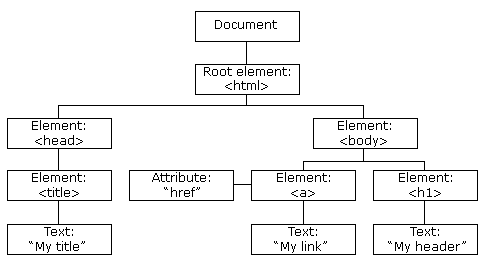
\includegraphics[keepaspectratio=true, width=14cm]{images/javascript/html_dom.png}
\resizebox{16cm}{!}{
	\fdot[scale=0.8]{images/dom}{--autosize}
}
\caption{Baumstruktur des HTML-DOM}
\end{figure}

Durch dieses Modell und zusätzliche Funktionen, welche als Bibliothek (z.B. jQuery), eingebunden werden können, kann man mit JavaScript die einzelnen Elemente einer Webseite verändern. Das kann genutzt werden um nachträglich geladene Inhalte in die Webseite einzubauen, oder das aussehen der Webseite zu verändern ohne diese neu zu laden.\\
Als Ergänzung zum DOM gibt es noch ein BOM (Browser Object Model). Die Objekte aus denen dieses Modell besteht, geben dann zum Beispiel die Fensterhöhe oder Fensterbreite an, es werden aber auch Informationen über das verwendete Betriebssystem und den verwendeten Browser angegeben.

\paragraph{JSON}
JavaScript Object Notation ist ein Datenaustauschformat welches so gestaltet ist, dass Objekte als Text codieren kann und der Computer es einfach parsen kann. Es basiert auf JavaScript.\\
JSON wird sehr häufig in Verbindung mit JavaScript verwendet, kann aber auch mit anderen Programmiersprachen verwendet werden.\\
Beispiel für ein JSON-Objekt:\\
\begin{lstlisting}[language=html]
{
  "Gerät": "Auto",
  "Marke": "Audi",
  "Farbe": "rot",
  "Seriennummer": 02345032,
}
\end{lstlisting}
Die Daten werden in Form von Daten-Wert Paaren gespeichert. Aus diesem Objekt kann man nur relativ einfach Daten auslesen.\\ 



